\documentclass{article}
%packages
\usepackage{graphicx}
\usepackage[latin1]{inputenc}
\usepackage[T1]{fontenc}
\usepackage[frenchb]{babel}
\usepackage[a4paper]{geometry}

\begin{document}
%title
\begin{titlepage}
	\vspace{-20px}
	\begin{tabular}{l}
		\textsc{Blin} S\'ebastien\\
		\textsc{Collin} Pierre-Henri
	\end{tabular}
	\hfill \vspace{10px}
\includegraphics[scale=0.1]{esir.png}\\
	\vfill
	\begin{center}
		\Huge{\'Ecole sup\'erieure d'ing\'enieurs de Rennes}\\
		\vspace{1cm}
		\LARGE{1\`ere Ann\'ee}\\
		\large{Parcours Informatique}\\
		\vspace{0.5cm}\hrule\vspace{0.5cm}
		\LARGE{\textbf{BDD}}\\
		\Large{Compte-Rendu TP1,2,3}
		\vspace{0.5cm}\hrule
		\vfill
		\vfill
	\end{center}
	\begin{flushleft}
		\Large{Sous l'encadrement de~:}\\
		\vspace{0.2cm}
		\large{{Zoltan} Miklos}
	\end{flushleft}
	\vfill
\end{titlepage}

\section{TP1}
\subsection{Exercice 1}
Cr\'eation d'une base de donn\'ees de trois tables : {\bfseries etudiant} (avec les attributs etuId, nom, prenom, adress), {\bfseries professeur} (avec les attributs profId, nom, prenom) et {\bfseries enseignement} (avec les attributs ensId, sujet, etuId, profId).\\
\begin{verbatim}
sqlite> CREATE TABLE etudiant (etuId INT PRIMARY KEY, nom varchar(255),
prenom varchar(255), adress varchar(255));
sqlite> CREATE TABLE professeur (profId INT PRIMARY KEY, nom varchar(255),
prenom varchar(255));
sqlite> CREATE TABLE enseignement (ensId INT PRIMARY KEY, sujet varchar(255),
etuId INT REFERENCES etudiant, profId INT REFERENCES professeur);
\end{verbatim}
Insertion de quelques enregistrements dans les tables :
\begin{verbatim}
INSERT INTO etudiant VALUES(1, "Martin", "Georges",
 "45 avenue de la Victoire 35000 Rennes");
INSERT INTO etudiant VALUES(2, "Durand", "Laura",
 "9 rue des Abeilles 44000 Nantes");
INSERT INTO etudiant VALUES(3, "Roux", "Bertrand",
 "16 rue Leon Blum 35000 Rennes");
INSERT INTO etudiant VALUES(4, "Dubois", "Valerie",
 "178 Boulevard Saint-Germain 75000 Paris";
INSERT INTO etudiant VALUES(5, "Fontaine", "Patrice",
 "56 allee des Camelias 29200 Brest");
INSERT INTO professeur VALUES(1, "Martinez", "Fabrice");
INSERT INTO professeur VALUES(2, "Lambert", "Andre");
INSERT INTO enseignement VALUES(1, "Base de donnees", 1, 1);
INSERT INTO enseignement VALUES(1, "Base de donnees", 2, 1);
INSERT INTO enseignement VALUES(3, "Base de donnees", 3, 1);
INSERT INTO enseignement VALUES(4, "Systeme", 4, 2);
INSERT INTO enseignement VALUES(5, "Systeme", 5, 2);
\end{verbatim}
Quelques exemples de requ\^etes SQL : \\\\
Liste des noms des \'etudiants qui suivent le cours {\bfseries Base de donn\'ees}
\begin{verbatim}
SELECT nom 
FROM etudiant etu, enseignement ens 
WHERE ens.sujet="Base de donnees" AND etu.etuId=ens.etuId;
Martin
Durand
Roux
\end{verbatim}
Liste des pr\'enoms des professeurs de l'\'etudiant {\bfseries Georges}
\begin{verbatim}
SELECT prof.prenom 
FROM etudiant etu, enseignement ens, professeur prof 
WHERE etu.prenom="Georges" AND etu.etuId=ens.etuId AND ens.profId=prof.profId;
Fabrice
\end{verbatim}
\subsection{Exercice 3}
V\'erification des r\'eponses du TD1 :\\\\
Question 1:
\begin{verbatim}
SELECT nom_p 
FROM Produit 
WHERE origine="Dijon";
\end{verbatim}
Question 2:
\begin{verbatim}
SELECT F.f, F.nom_f 
FROM Fournisseur F, Produit P, Fourniture Ft 
WHERE F.f=Ft.f AND P.p=Ft.p AND P.nom_p="Salade";
\end{verbatim}
Question 3:
\begin{verbatim}
SELECT P.p 
FROM Produit P, Fournisseur F, Fourniture Ft 
WHERE F.f=Ft.f AND P.p=Ft.p AND F.ville="Paris";
\end{verbatim}
Question 4:
\begin{verbatim}
SELECT F.nom_f, F.remise 
FROM Fournisseur F 
EXCEPT
SELECT F.nom_f, F.remise
FROM Produit P, Fournisseur F, Fourniture Ft
WHERE F.f=Ft.f AND P.p=Ft.p AND P.origine="Dijon"; 
\end{verbatim}
Question 5:
\begin{verbatim}
SELECT nom_p 
FROM Fournisseur F, Produit P, Fourniture Ft 
WHERE F.f=Ft.f AND P.p=Ft.p AND qte<5 AND nom_f="Bornibus";
\end{verbatim}
Question 6:
\begin{verbatim}
SELECT nom_f, ville 
FROM Fournisseur A, Fournisseur B 
WHERE F.nom_f="Bornibus" AND A.remise > B.remise;
\end{verbatim}
Utilisation de la commande {\bfseries .read}
\begin{verbatim}
sqlite> .read td1.sql 
cassis
moutarde
cornichon
p1
p4
p5
p6
p2
p4
Dupont|0
Tanguy|10
cassis
moutarde
cornichon
Mercier|Paris
Bossuet|Dijon
Tanguy|Riec
\end{verbatim}
\begin{verbatim}
\end{verbatim}
\subsection{Exercice 4}
\begin{verbatim}
SELECT nom_f, nom_p
FROM Fournisseur fs, Produit p, Fourniture ft
WHERE fs.f=ft.f AND p.p=ft.p;
\end{verbatim}
\begin{verbatim}
Bornibus|cassis
Bornibus|moutarde
Bornibus|salade
Bornibus|cornichon
Mercier|champagne
Mercier|moutarde
Colbert|champagne
Colbert|moutarde
Bossuet|moutarde
Bossuet|salade
Bossuet|cornichon
Tanguy|muscadet
\end{verbatim}
Cette requ\^ete permet de connaitre les produits propos\'es par les fournisseurs
\begin{verbatim}
EXPLAIN QUERY PLAN SELECT nom_f, nom_p 
FROM Fournisseur fs, Produit p, Fourniture ft 
WHERE fs.f=ft.f AND p.p=ft.p;

0|0|0|SCAN TABLE Fournisseur AS fs
0|1|2|SEARCH TABLE Fourniture AS ft USING AUTOMATIC COVERING INDEX (f=?)
0|2|1|SEARCH TABLE Produit AS p USING AUTOMATIC COVERING INDEX (p=?)
\end{verbatim}
\section{TP2}
\subsection{But du TP}
Une entreprise enregistre ses transactions dans un fichier Excel qui est tr\`es dur \`a maintenir. On doit donc proposer une solution pour rendre la maintenance plus facile et \'eviter des pertes de donn\'ees.
\subsection{Solution propos\'ee}
Nous sommes donc partis sur une base de donn\'ees comprenant 3 tables :
\begin{itemize}
  \item Une base Client contenant un nom de client, un num\'ero de t\'el\'ephone, et une adresse. Ce qui \'evite la perte de client avec la suppression d'une facture.
  \item Une base Produit contenant un nom de produit, un prix d'achat et de vente (pour calculer les rabais) et un prix de TVA.
  \item Une base Facture contenant un num\'ero de facture, un client, un produit, une quantit\'e et une date.  
\end{itemize}
Ce qui nous donne en SQL :\\
\begin{verbatim}
sqlite TP2.db
CREATE TABLE Client (numC INT PRIMARY KEY, nomC TEXT, 
tel TEXT, address TEXT);
INSERT INTO Client VALUES(1, "Alpha CO", "1231231231", 
"3, rue du thabor, 35000 Rennes");
INSERT INTO Client VALUES(2, "Beta CO", "3213213213", 
"43, place de la republique, 35000 Rennes");
INSERT INTO Client VALUES(3, "Gamma CO", "7417417417", 
"32, rue d'orleans, 44000 Nantes");
CREATE TABLE Produit (numP INT PRIMARY KEY, nomP TEXT, 
prixVente FLOAT, prixAchat FLOAT, tva FLOAT);
INSERT INTO Produit VALUES(1, "pomme", 1, 0.2, 1);
INSERT INTO Produit VALUES(2, "tomate", 0.5, 0.1, 2);
INSERT INTO Produit VALUES(3, "orange", 1, 0.2, 2);
CREATE TABLE Facture (num INT PRIMARY KEY, numC INT 
REFERENCES Client, numP INT REFERENCES Produit, qte INT,
date TEXT);
INSERT INTO Facture VALUES(123, 1, 1, 2, "2.3.2013");
INSERT INTO Facture VALUES(124, 2, 2, 22, "3.4.2013");
INSERT INTO Facture VALUES(125, 3, 3, 13, "4.4.2013");
SELECT * FROM Facture f, Client c, Produit p WHERE 
f.numC = c.numC AND f.numP = p.numP;
123|1|1|2|2.3.2013|1|Alpha CO|1231231231|3, rue du 
thabor, 35000 Rennes|1|pomme|1|1
124|2|2|22|3.4.2013|2|Beta CO|3213213213|43, place de 
la republique, 35000 Rennes|2|tomate|0.5|2
125|3|3|13|4.4.2013|3|Gamma CO|7417417417|32, rue 
d'orleans, 44000 Nantes|3|orange|1|2
\end{verbatim}
\subsection{Quelques requ\^etes}
Ces 3 tables nous permettent de facilement trouver les clients habitant \`a Rennes :\\
\begin{verbatim}
SELECT nomC 
FROM Client 
WHERE address LIKE '%Rennes';
Alpha CO
Beta CO
\end{verbatim}
Nous pouvons obtenir le prix total de chaque facture avec :
\begin{verbatim}
SELECT prix*qte+tva 
FROM Facture f, Client c, Produit p 
WHERE f.numC = c.numC AND f.numP = p.numP;
3
13
15
\end{verbatim}
Retrouver le plus gros client, avec une requ\^ete imbriqu\'ee qui recherche le nom du client avec la plus grosse commande (On aurait pu faire un GROUP BY Client, mais on a choisi de chercher la plus grosse facture).
\begin{verbatim}
SELECT C.nomC 
FROM Facture f, Client c, Produit p 
WHERE f.numC = c.numC AND f.numP = p.numP AND prix*qte+tva = 
  (SELECT MAX(prix*qte+tva) 
  FROM Facture f, Client c, Produit p 
  WHERE f.numC = c.numC AND f.numP = p.numP);
Gamma CO
\end{verbatim}
Nous pouvons aussi facilement modifier les prix des produits (ce qui change le prix des factures pass\'ees, vu que nous avons d\'ecid\'e de ne pas en garder la trace. Il aurait fallu rajouter un prix total calcul\'e automatiquement d\`es l'arriv\'ee de la facture (TRIGGER)). Ainsi que modifier les tables facilement (ajout d'un client, d'un produit, d'une facture ou suppression) :
\begin{verbatim}
Le prix des oranges a baisse de 10%
sqlite> SELECT * FROM Produit;
1|pomme|1|0.2|1
2|tomate|0.5|0.1|2
3|orange|1|0.2|2
sqlite> UPDATE Produit SET prixVente = prixVente -0.1*prixVente WHERE 
nomP = "orange";
sqlite> SELECT * FROM Produit;
1|pomme|1|0.2|1
2|tomate|0.5|0.1|2
3|orange|0.9|0.2|2

INSERT INTO Produit VALUES(4, "Kiwi", 1, 0.2, 2);
DELETE FROM Produit WHERE nomP = "Kiwi";
\end{verbatim}
Rabais maximal par facture
\begin{verbatim}
SELECT num, qte*prixVente - qte*prixAchat 
FROM Facture f, Produit p 
WHERE f.numP = p.numP;
123|1.6
124|8.8
125|9.1
\end{verbatim}
Le rabais maximum possible pour le client qui a pay\'e la plus grosse facture.
\begin{verbatim}
sqlite> SELECT c.nomC, num, qte*prixVente - qte*prixAchat 
FROM Facture f, Produit p, Client c 
WHERE f.numP = p.numP AND f.numC = c.numC AND f.numC = 
  (SELECT c.numC 
  FROM Facture f, Client c, Produit p 
  WHERE f.numC = c.numC AND f.numP = p.numP AND prixVente*qte+tva = 
    (SELECT MAX(prixVente*qte+tva) 
    FROM Facture f, Client c, Produit p 
    WHERE f.numC = c.numC AND f.numP = p.numP));
Gamma CO|125|9.1
\end{verbatim}

\section{TP3}
\subsection{But du TP}
Le but de ce TP est de montrer \`a quel point les index sont utiles et am\'eliorent la vitesse des requ\^etes lorsqu'ils sont bien choisis.
\subsection{Les index}
Dans cette partie du TP nous avons d\^u regarder le temps mis \`a ex\'ecuter 2 requ\^etes avec et sans index. Sans index, les 2 requ\^etes s'ex\'ecutaient en environ 1.5 secondes. Avec index, le temps mis \`a calculer les requ\^etes est quasiment nul.
\subsection{Optimisation}
Dans cette partie, nous avons remarqu\'e que les jointures (naturelles et \`a l'aide de FROM A,B) \'etaient plus longues \`a \'evaluer que les requ\^etes imbriqu\'ees.\\
\'A l'aide de la commande CREATE INDEX, nous avons alors mis un index sur l'attribut id de la table customer.\\
Le temps a \'et\'e consid\'erablement r\'eduit.\\\\
\begin{center}
\begin{tabular}{|l|c|r|}
  \hline
   & Sans Index & Avec Index \\
  \hline
  1 & 11,0552 & 0,2206 \\
  \hline
  2 & 0,542 & 0,2138 \\
  \hline
  3 & 11,0448 & 0,2176 \\
  \hline
  4 & 8,2936 & 0,2142 \\
  \hline
\end{tabular}\\
\end{center}\\
Nous avons pu r\'ealiser quelques graphiques pour montrer l'am\'elioration apport\'ee par les index. Ainsi que les optimisations apport\'ees par ceux-ci (le temps d'ex\'ecution des 4 requ\^etes est identique).\\
\begin{figure}
	\begin{center}
		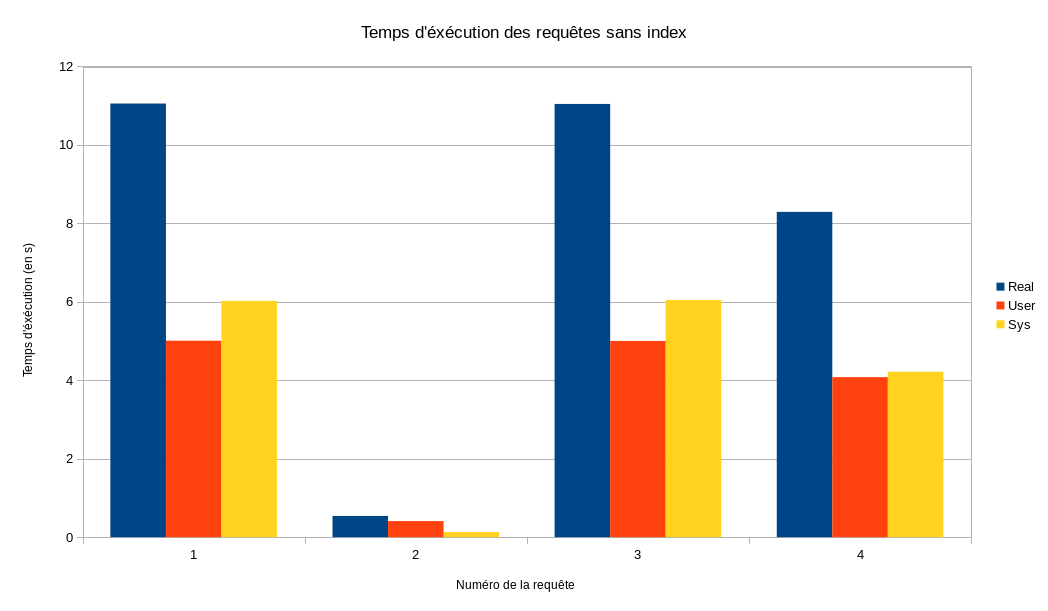
\includegraphics[scale=0.55]{images/rsi}\\
		Temps d'\'ex\'ecution des requ\^etes sans index
	\end{center}
\end{figure}
\begin{figure}
	\begin{center}
		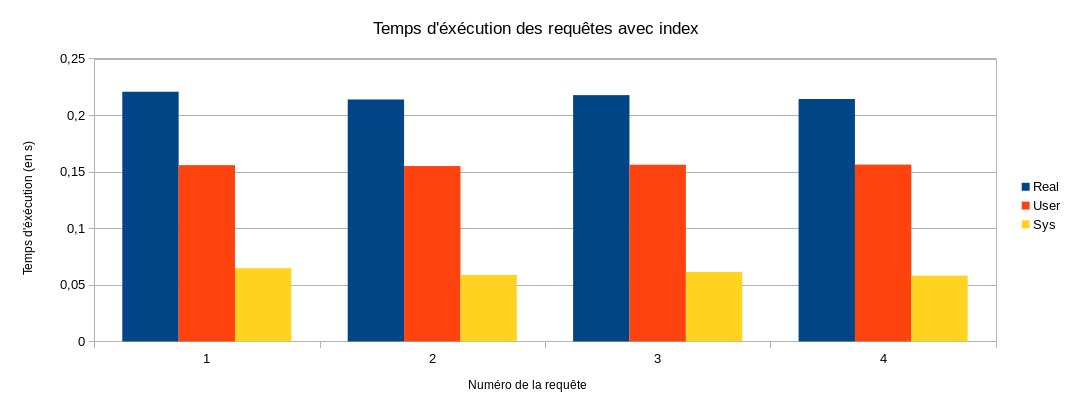
\includegraphics[scale=0.55]{images/rai}\\
		Temps d'\'ex\'ecution des requ\^etes avec index
	\end{center}
\end{figure}
\begin{figure}
	\begin{center}
		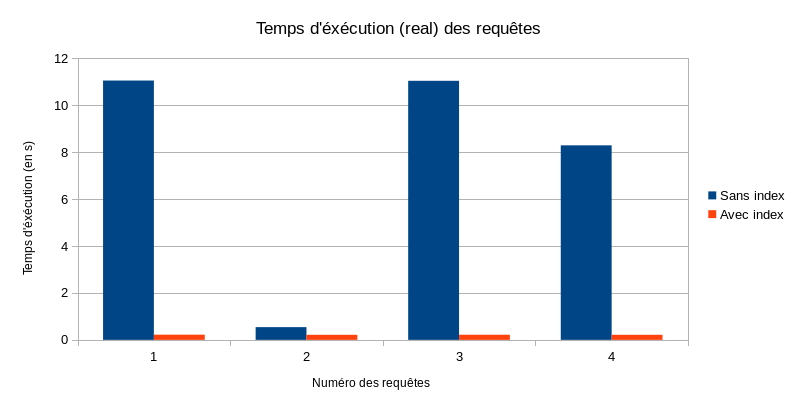
\includegraphics[scale=0.7]{images/siai}\\
		Temps d'\'ex\'ecution avec et sans index
	\end{center}
\end{figure}
\end{document}

